\chapter{Vervolg op bachelorproef}
\label{ch:Vervolg op bachelorproef}

\section{Verwerken van SDSF output}
\label{sec:Verwerken van SDSF output}

Een interessant vervolg van deze proef is het maken van applicaties/programma's voor het beheer van SDSF. En voornamelijk het beheer van het Health Checker panel. Een vervolg op deze proef zou een vergelijkende studie kunnen zijn tussen Java en REXX en de manier waarop ze met SDSF data kunnen werken.

\subsection{REXX vs Java}
\label{subsec:REXX vs Java}



REXX(Restructured Extendend Executor) is een programmeertaal ontworpen door IBM. Deze taal wordt ook gebruikt op de mainframe. Maar wat ook belangrijk is is dat deze taal gebruikt kan worden op programma's te schrijven die werken met SDSF. Dit doe je met de REXX met SDSF interface. Hiermee kan je via REXX meerdere panelen aanroepen en bepaalde kolommen tonen. Rexx kan zelf gebruikt worden om grafieken te maken van data uit SDSF. Of om jobs uit te voeren. (\cite{Parziale2007})

Java is nog een andere taal die gebruikt kan worden. Met de SDSF Java API kan je SDSF data verwerken via een java programma. De API laat je toe om de verschillende SDSF panelen en hun bijhorende data op te vragen. Met java kan je ook acties uitvoeren zoals de kolom commando's in SDSF. Hiermee zou je een check mee kunnen starten bijvoorbeeld. (\cite{Wood2012})

Een vervolg op de proef zou een studie kunnen zijn die onderzoekt welke van de 2 opties het meest geschikt zou zijn voor het verwerken van SDSF Data. En de taal die het meest geschikt zou zijn voor interactie met z/OS Health checker via SDSF



\section{Web Interface}
\label{sec:Web interface}

HCL Technologies hun logging is gewenst via mail. Maar het zou interessant zijn om de logging van z/OS Health Checker uit te breiden naar een WebUI. Daarom worden er in dit hoofdstuk nog methoden bekeken om de SDSF output te loggen op een webpagina. Om webpagina's te hosten op z/OS zijn enkele mogelijkheden. Dit kan zowel voor statische webpagina's maar dynamische webpagina's zijn degene die nodig zijn. Een van de manieren voor een dynamische website te hosten op z/OS is met volgende setup.

De setup bevat een z/OS HTTP web server met een Webpshere application Server plug-in. In deze plugin zit een java servlet dit is een java programma dan interactie heeft met de EJB. Dit staat voor Enterprise JavaBeans dit is een server side software component. Deze draait dan op een J2EE server. (\cite{IBM2010})

Deze server bied een platform aan voor server side applicaties. En aangezien interactie mogelijk is tussen Java en SDSF met de SDSF Java API. Zou je dus zo de SDSF output op een webpagina krijgen. En zo een logging systeem maken met een webUI. (\cite{Vilaghy2002})

\begin{figure}[h]
	\centering
	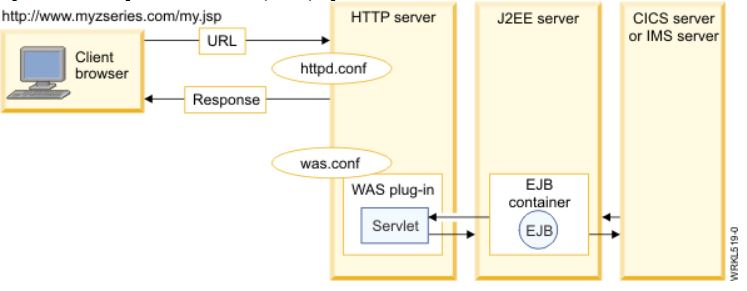
\includegraphics{img/WebpshereApplicationServer}
	\caption[Websphere Application Server]{Visualisatie van de omgeving nodig voor het draaien van dynamische webpagina's op z/OS(\cite{IBM2010})}
	\label{fig:webpshereapplicationserver}
\end{figure}


Een vervolg van deze proef kan dus een studie zijn naar het opzetten van deze architectuur en de mogelijkheden die ze bied voor het werken met SDSF via een webUI.





